\numberedsection{RF5.3 Editar relación}

\subsection*{Descripción}
Permite a los usuarios modificar los datos de las relaciones existentes.\par
\vspace{0.15cm}

\textbf{Pre-condición}\par
El usuario ha iniciado sesión en su cuenta en Mini PIM y la relación a editar existe en el sistema.\par
\vspace{0.15cm}

\textbf{Post-condición}
\begin{itemize}
    \item Caso de éxito: El sistema actualiza los datos de la relación seleccionada y refleja los cambios en la lista de relaciones.
    \item Caso mínimo: El sistema notifica al usuario el resultado de la acción de edición de la relación: exitosa o fallida.
\end{itemize}

\textbf{Prioridad: }
Media
\vspace{0.15cm}

\textbf{Autor: }
Pablo Ortega Serapio\par
\vspace{0.15cm}

\textbf{Control de cambios: } Versión 1: Definición del caso de uso

\numberedsubsection{Escenario principal}
\begin{enumerate}
    \item El usuario ha iniciado sesión con su cuenta de usuario correspondiente.
    \item El usuario accede a la sección de \enquote{Relaciones}.
    \item El sistema muestra la lista de relaciones existentes y la opción para editar una relación.
    \item El usuario selecciona una relación y la opción de editar una relación existente.
    \item El sistema presenta un menú con el nombre actual de la relación y dos columnas con todos los productos.
    \item El usuario hace los cambios que considere en el nombre y la selección de productos\footnote{Se le permite al usuario cambiar el nombre previamente asignado a la relación, añadir nuevos productos a la selección actual o quitar productos de la relación previamente escogidos.}.
    \item El usuario selecciona \enquote{Confirmar} para guardar las modificaciones.
    \item El sistema verifica que el nombre de la relación no sea erróneo.
    \item El sistema verifica que si se selecciona un producto de la columna izquierda, también debe haber un producto seleccionado en la columna derecha.
    \item El sistema muestra la lista de relaciones con los cambios realizados.
\end{enumerate}

\numberedsubsection{Escenarios alternativos}
\begin{description}
    
    \item[7.a] El sistema detecta que el nombre de la relación es erróneo.
    \begin{enumerate}
        \item[7.a.1] El sistema muestra un mensaje de error indicando que el nombre no es válido.
        \item[7.a.2] El sistema devuelve al usuario al menú de creación de relación permitiendo modificar el nombre.
    \end{enumerate}
    
    \item[8.a] El sistema detecta que solo hay elementos seleccionados en la columna izquierda.
    \begin{enumerate}
        \item[8.a.1] El sistema muestra un mensaje de error solicitando que seleccione un producto de la tabla derecha o que se deseleccionen los productos de la columna izquierda.
        \item[8.a.2] El sistema devuelve al usuario al menú de creación de relación para continuar eligiendo productos.
    \end{enumerate}

    \item[*.a] El usuario cancela la acción de editar la relación seleccionada cerrando el menú de creación de relación.
    \begin{enumerate}
        \item[*.a.1] El sistema regresa a la sección de \enquote{Relaciones}.
    \end{enumerate}
\end{description}

\numberedsubsection{Casos de Prueba}
\underline{Escenario: Principal}\par
\vspace{0.15cm}
\textbf{Dado} que el usuario ha iniciado sesión con su cuenta de usuario correspondiente,\par
\textbf{Y} se encuentra en el apartado de \enquote{Relaciones},\par
\textbf{Cuando} selecciona la opción de \enquote{Editar} para modificar una relación existente,\par
\textbf{Y} el sistema presenta un menú de edición con el nombre actual de la relación, y dos columnas con los productos a relacionar,\par
\textbf{E} el usuario introduce correctamente el nombre de la relación que desea editar,\par
\textbf{Y} selecciona correctamente los productos en las columnas,\par
\textbf{Y} selecciona \enquote{Confirmar} para guardar los datos,\par
\textbf{Entonces} el sistema actualiza la información de la relación,\par
\textbf{Y} actualiza la lista de relaciones con la relación modificada,\par
\textbf{Y} muestra el apartado de relaciones con todas las relaciones almacenadas.\par

\vspace{0.20cm}

\underline{Escenario: Alternativo 7.a (nombre de relación erróneo)}\par
\vspace{0.15cm}

\textbf{Dado} que el usuario ha iniciado sesión con su cuenta de usuario correspondiente,\par
\textbf{Y} se encuentra en el apartado de \enquote{Relaciones},\par
\textbf{Cuando} selecciona la opción de \enquote{Editar},\par
\textbf{Y} rellena el campo de nombre de la relación de forma errónea,\par
\textbf{Entonces} el sistema notifica al usuario que el campo de nombre es erróneo,\par
\textbf{Y} muestra un mensaje de error y lo devuelve al menú para continuar creando la relación.\par

\vspace{0.20cm}

\underline{Escenario: Alternativo 8.a (productos no seleccionados correctamente)}\par
\vspace{0.15cm}

\textbf{Dado} que el usuario ha iniciado sesión con su cuenta de usuario correspondiente,\par
\textbf{Y} se encuentra en el apartado de \enquote{Relaciones},\par
\textbf{Cuando} selecciona la opción de \enquote{Añadir relación},\par
\textbf{Y} selecciona los productos de forma errónea,\par
\textbf{Entonces} el sistema notifica al usuario que ha seleccionado los productos de forma errónea,\par
\textbf{Y} muestra un mensaje de error y lo devuelve al menú para continuar creando la relación.\par

\vspace{0.20cm}

\underline{Escenario: Alternativo *.a (cancelar la acción de editar relación)}\par
\vspace{0.15cm}
\textbf{Dado} que el usuario ha iniciado sesión con su cuenta de usuario correspondiente,\par
\textbf{Y} se encuentra en el apartado de \enquote{Relaciones},\par
\textbf{Cuando} selecciona una relación para \enquote{Editar},\par
\textbf{Y} decide cancelar la acción de edición cerrando el menú,\par
\textbf{Entonces} el sistema regresa a la sección \enquote{Relaciones},\par
\textbf{Y} muestra la lista de relaciones sin realizar ningún cambio.\par


\newpage % Muestra los bocetos en una nueva página

\numberedsubsection{Bocetos}
\begin{figure}[H]
    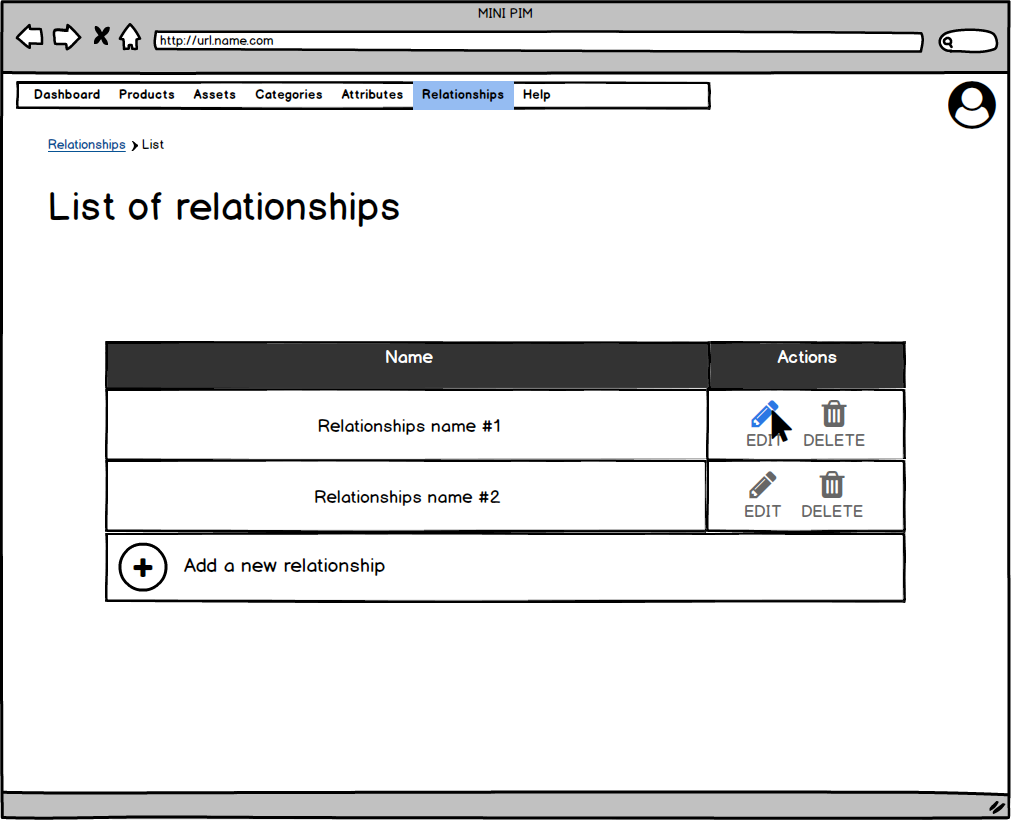
\includegraphics[width=1\linewidth]{assets/mockups/RF5.3_1.png}
    \caption{Se desea editar la relación 1}
   \end{figure}
\vspace{1.0cm}

\begin{figure}[H]
    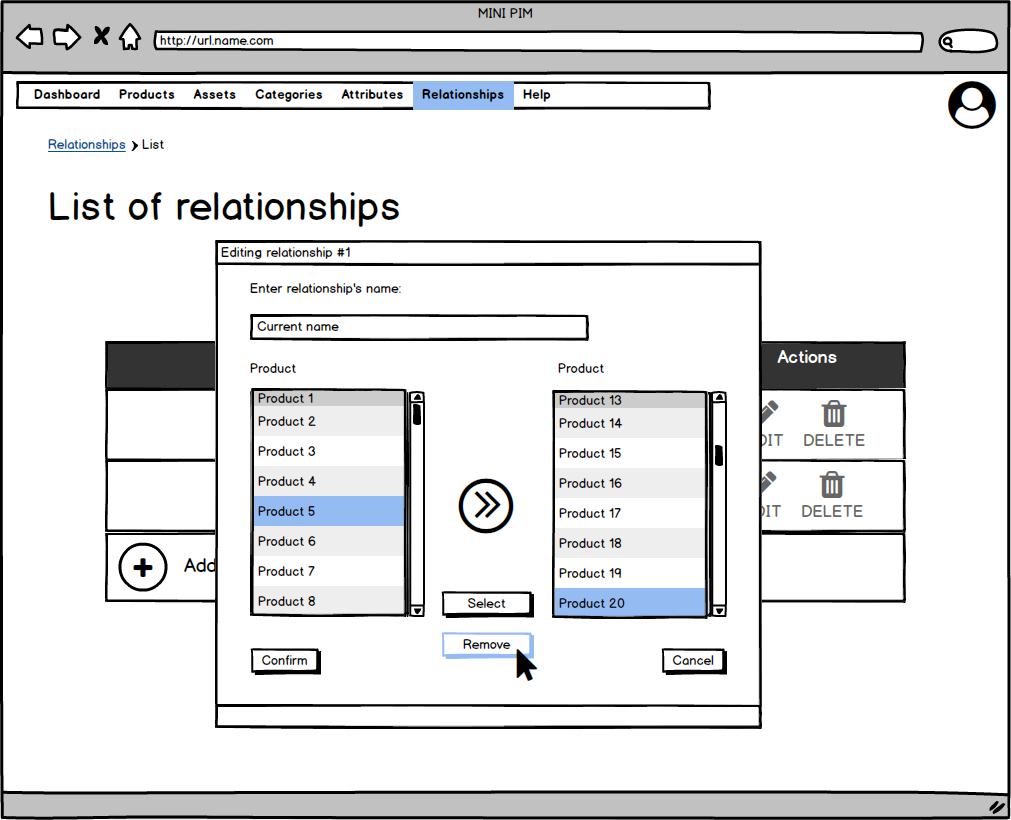
\includegraphics[width=1\linewidth]{assets/mockups/RF5.3_2.png}
    \caption{Menú de edición para la relación seleccionada}
   \end{figure}
\vspace{1.0cm}

\newpage % Muestra el diagrama de secuencias en una nueva página

\numberedsubsection{Diagrama de Secuencia (por hacer)}
\begin{figure}[H]
    
\includegraphics[width=1\linewidth]{assets/umaLogo.png}
    \caption{Escenario principal para crear el Informe de Cuenta}
   \end{figure}
\vspace{1.0cm}

\newpage % Inicia en una nueva página otro caso de uso